% !TeX root = RJwrapper.tex
\title{freesurfer: Connecting the Freesurfer Software with R}
\author{by John Muschelli, Elizabeth M. Sweeney, Ciprian M. Crainiceanu}

\maketitle

\abstract{%
We present the package \CRANpkg{freesurfer}, a set of R functions that
interface with Freesurfer, a commonly-used open-source software package
for processing and analyzing structural neuroimaging data, specifically
T1-weighted images. The \pkg{freesurfer} package performs operations on
\code{nifti} image objects in R using command-line functions from
Freesurfer, and returns R objects back to the user. \pkg{freesurfer}
allows users to process neuroanatomical images and provides
functionality to convert and read the output of the Freesurfer pipelines
more easily.
}

\section{Introduction}\label{introduction}

\label{sec:intro}

Freesurfer is a commonly-used software for processing and analyzing
anatomical neuroimaging data \citep{fischl2012freesurfer}, developed by
the Laboratory for Computational Neuroimaging at the Athinoula A.
Martinos Center for Biomedical Imaging. This software provides
open-source, command-line tools for image processing tasks such as brain
extraction/skull-stripping \citep{segonne2004hybrid}, bias-field
correction \citep{sled_nonparametric_1998}, segmentation of structures
within the brain \citep{fischl2002whole,fischl2004sequence}, and image
registration \citep{fischl1999high,reuter2010highly}. In additio to
these functions, Freesurfer has functions that perform complete
pipelines for the user.

We have previously published a similar adaptation of the FSL imaging
software \citep{jenkinson_fsl_2012} to R, called \CRANpkg{fslr}
\citep{muschelli2015fslr}. Again, we note that there exist a number of R
packages for reading and manipulating image data, including
\CRANpkg{AnalyzeFMRI} \citep{bordier_temporal_2011}, \CRANpkg{RNiftyReg}
\citep{modat_rniftyreg:_2013}, and \CRANpkg{fmri}
\citep{tabelow_statistical_2011} (see the Medical Imaging CRAN task view
\url{http://cran.r-project.org/web/views/MedicalImaging.html} for more
information). Although these packages are useful for performing image
analysis, much of the functionality of image processing that Freesurfer
provides are not currently implemented in R, including surface-based
registration. The \pkg{ANTsR} package
(\url{https://github.com/stnava/ANTsR}) is a currently unpublished R
package that interfaces with the ANTs (advanced normalization tools)
software suite \citep{avants_reproducible_2011}, where a lot of
additional functionality has been implemented, but this package has not
been released onto CRAN. Moreover, having multiple options for image
processing through R allows for users to compare methods and the
flexibility of using multiple packages to achieve a working data
processing pipeline.

In particular, we provide an interface to users to the state-of-the-art
anatomical processing implemented in Freesurfer, as well as a suite of
tools that simplify analyzing the output of Freesurfer. The
\pkg{freesurfer} allow R users to implement complete anatomical imaging
analyses without necessarily learning Freesurfer-specific syntax.

\subsection{\texorpdfstring{Imaging formats in \pkg{freesurfer} and
R}{Imaging formats in  and R}}\label{imaging-formats-in-and-r}

The \CRANpkg{freesurfer} package relies on the \CRANpkg{oro.nifti}
\citep{whitcher_working_2011} package implementation of images (referred
to as \code{nifti} objects) that are in the Neuroimaging Informatics
Technology Initiative (NIfTI) format, as well as other common image
formats such as ANALYZE. Some Freesurfer functions require other
formats, such as MINC
(\url{http://www.bic.mni.mcgill.ca/ServicesSoftware/MINC}). The
Freesurfer installation provides functions to convert from MINC to NIfTI
formats and there are implemented in functions such as \code{nii2mnc}
and \code{mnc2nii} in R. Moreover, the \code{mri\_convert} Freesurfer
function has been interfaced in the \code{freesurfer} package (same
function name), which allows for a more general conversion tool of
imaging types for R users than currently implemented in native R. Thus,
many formats can be converted to NIfTI and then read into R using the
\code{readNIfTI} function from \pkg{oro.nifti}.

\subsection{Reconstruction pipeline in
Freesurfer}\label{reconstruction-pipeline-in-freesurfer}

The Freesurfer pipeline and analysis workflow for neuroanatomical images
is based on a structural magnetic resonance image (MRI) of the brain.
The specific type of image commonly used in this software is a
T1-weighted image, a specific MRI sequence commonly taken. The full
pipeline is implemented in the Freesurfer \code{recon-all} function,
where the ``recon'' stands for reconstruction
(\url{https://surfer.nmr.mgh.harvard.edu/fswiki/recon-all}). Using the
\code{-all} flag in the the \code{recon-all} function performs over 30
different steps and takes 20-40 hours to fully process a subject when
performing all the steps. This process is the common way of fully
processing an T1-weighted image in Freesurfer, and is implemented in the
\texttt{recon\_all} \pkg{freesurfer} function.

If there are problems with the result of this processing, there are
multiple steps users can edit certain parts of the processing, such as
skull-stripping, where non-brain tissues are removed from the image. The
remainder of the pipeline can be run after these steps. The full
pipeline is broken down into 3 separate steps, referred to as
\code{autorecon1}, \code{autorecon2}, and \code{autorecon3}, which
correspond to the flags in \code{recon-all} used to initiate these
steps. We have written wrapper functions \code{autorecon1},
\code{autorecon2}, and \code{autorecon3}, respectively, for simplicity
to the R user. This allows users to run pieces of the pipeline if
desired or restart a failed process after correction to the data.

\subsection{R function setup}\label{r-function-setup}

To use \pkg{freesurfer}, a working installation of Freesurfer is
required. The following code was run using Freesurfer version
``freesurfer-Darwin-lion-stable-pub-v5.3.0''. The Freesurfer version can
be accessed using the \code{fs\_version} function. \pkg{freesurfer} must
also have the path of Freesurfer specified. If using R from a shell
environment, and the \code{FREESURFER\_HOME} environment variable is set
(which can be done when installing Freesurfer), \pkg{freesurfer} will
use this as the path to Freesurfer. If using R through a graphical user
interface (GUI) such as RStudio (RStudio, Boston, MA), environmental
variables and paths are not explicitly exported. Therefore,
\code{FREESURFER\_HOME} is not set, \pkg{freesurfer} will try the
default directories of Mac OSX and Linux. If the user did not perform an
standard installation of Freesurfer, the path to Freesurfer can be
specified using \code{options(freesurfer.path="/path/to/freesurfer")}.

We will discuss the setup functions for the \pkg{freesurfer} package and
how they can be used in analysis and example code. For testing, whether
a user has a Freesurfer installation, the \code{have\_fs} function
provides a logical indicator as a result. The \code{fs\_dir} function
will return the directory of the Freesurfer installation.

\subsubsection{Structure of Freesurfer
analyses}\label{structure-of-freesurfer-analyses}

During the installation of Freesurfer, a series of variables are set up
in the user's shell environment. One of these variables is
\code{SUBJECTS\_DIR}, which refers to a directory of the output of
analysis from all subjects. This setup allows users to simply specify a
subject identifier to analyze, rather than a specific path or multiple
intermediate files.

This setup may not be desirable if the user prefers to structure the
data from multiple studies into different folders. For example, the
\code{asegstats2table} function takes the \textbf{a}natomical
\textbf{seg}mentation \textbf{stat}istics and convert it to a table. The
default argument for \code{asegstats2table} is to pass in a subject name
rather than a file. The \pkg{freesurfer} \code{asegstats2table} function
allows the R user to specify a different subject directory to read in
the file, while not overriding the default set by \code{SUBJECTS\_DIR}.
This functionality allows users to have separate folders with subjects
and read in the data by simply switching the \code{subj\_dir} argument
in the R function.

Similarly to the \code{fs\_dir} function, the \code{fs\_subj\_dir}
function will return the path to the Freesurfer subjects directory if it
is set.

Some Freesurfer functions require an image as an input. For those
functions, the R \pkg{freesurfer} functions that call those Freesurfer
functions will take in a file name or a \code{nifti} object. The R code
will convert the \code{nifti} to the corresponding input required for
Freesurfer. From the user's perspective, the input/output process is all
within R. The advantage of this approach is that the user can read in an
image, do manipulations of the \code{nifti} object using standard syntax
for arrays, and pass this object into the \pkg{freesurfer} R function.
Thus, users can use R functionality to manipulate objects while
seamlessly passing these object to Freesurfer through \pkg{freesurfer}.

\section{Example analyses and use of
functions}\label{example-analyses-and-use-of-functions}

In the default subjects directory in the Freesurfer installation, there
is a subject named ``bert'', where \code{recon-all} was run. A user can
see the result of this output in the ``bert'' directory:

\begin{Schunk}
\begin{Sinput}
list.files(path  = file.path(fs_subj_dir(), "bert"))
\end{Sinput}
\begin{Soutput}
 [1] "bem"     "label"   "mri"     "scripts" "src"     "stats"   "surf"   
 [8] "tmp"     "touch"   "trash"  
\end{Soutput}
\end{Schunk}

We will explore the results in ``mri'', which contain imaging data,
``stats'', which containing statistics based on structures of the brain,
and ``surf'', which contain the surface and curvature output from the
Freesurfer processing.

\subsection{Reconstruction}\label{reconstruction}

For the \texttt{recon\_all} function, users must specify the input file
(a T1-weighted image), the output directory, and the subject identifier.
This function will take 20-40 hours to fully process the input file.

\begin{Schunk}
\begin{Sinput}
recon_all(infile, outdir, subjid)
\end{Sinput}
\end{Schunk}

\subsubsection{Reading in anatomical
statistics}\label{reading-in-anatomical-statistics}

The ``aseg.stats'' in the ``stats'' folder of subject bert corresponds
to measures and statistics from the anatomical segmentation. The
\code{read\_aseg\_stats} function reads this corresponding file and
creates a list of 2 different \code{data.frame}s:

\begin{Schunk}
\begin{Sinput}
file = file.path(fs_subj_dir(), "bert", "stats", "aseg.stats")
out = read_aseg_stats(file)
names(out)
\end{Sinput}
\begin{Soutput}
[1] "measures"   "structures"
\end{Soutput}
\end{Schunk}

The \code{measures} element corresponds to global measurements of the
brain (e.g.~volume of the brain) as well as measures of gross anatomical
structures (e.g.~gray matter).

\begin{Schunk}
\begin{Sinput}
head(out$measures[, c("meaning", "value", "units")])
\end{Sinput}
\begin{Soutput}
                                                 meaning          value
1                              brain segmentation volume 1193318.000000
2           brain segmentation volume without ventricles 1174082.000000
3 brain segmentation volume without ventricles from surf 1173867.217735
4            left hemisphere cortical gray matter volume  237947.199463
5           right hemisphere cortical gray matter volume  238312.856735
6                      total cortical gray matter volume  476260.056198
  units
1  mm^3
2  mm^3
3  mm^3
4  mm^3
5  mm^3
6  mm^3
\end{Soutput}
\end{Schunk}

In some imaging analyses, comparing at these large measures of brain volume over time or across groups are of interest.  

The \code{structures} element corresponds to a set of measures and statistics for a set of fixed anatomical structures.

\begin{Schunk}
\begin{Sinput}
head(out$structures)
\end{Sinput}
\begin{Soutput}
  Index SegId NVoxels Volume_mm3                   StructName normMean
1     1     4    6563     6562.6       Left-Lateral-Ventricle  36.0959
2     2     5     228      228.3            Left-Inf-Lat-Vent  54.8842
3     3     7   15708    15708.2 Left-Cerebellum-White-Matter  92.7562
4     4     8   58536    58535.7       Left-Cerebellum-Cortex  77.2709
5     5    10    8150     8150.4         Left-Thalamus-Proper  92.8386
6     6    11    3214     3213.7                 Left-Caudate  80.9591
  normStdDev normMin normMax normRange
1    12.2771      16      91        75
2    10.7839      22      87        65
3     5.5123      40     107        67
4     9.9521      17     142       125
5     7.0182      49     109        60
6     8.2079      49     105        56
\end{Soutput}
\end{Schunk}

Similarly with global measures, these structure-specific measures can be
used in analysis. Moreover, a large deviation in volume for a specific
subject may indicate atrophy of a structure or an indication of a
segmentation error.

\subsubsection{MRI conversion}\label{mri-conversion}

The typical output format from Freesurfer is MGH/MGZ format, which is
explained here:
\url{https://surfer.nmr.mgh.harvard.edu/fswiki/FsTutorial/MghFormat}. As
NIfTI formats are one of the most common formats and has been the common
format for analysis in the \pkg{oro.nifti} and \pkg{neurobase} packages,
it is useful to convert these files to a NIfTI format to use in R. The
\code{mri\_convert} Freesurfer function will be used for that. Here we
will use the T1-weighted image from the ``bert'' subject and convert it
to NIfTI, and read it into R:

\begin{Schunk}
\begin{Sinput}
library(freesurfer)
bert_dir = file.path(fs_subj_dir(), "bert")
t1_mgz = file.path(bert_dir, "mri", "T1.mgz")
t1_nii_fname = tempfile(fileext = ".nii.gz")
freesurfer::mri_convert(t1_mgz, t1_nii_fname)
img = neurobase::readnii(t1_nii_fname)
\end{Sinput}
\end{Schunk}

As this is a commonly-used function, we have wrapped these two steps
into the \texttt{readmgz} and \texttt{readmgh} functions, which warp
\texttt{mri\_convert} and \texttt{readnii}. Here we show that these
steps are equivalent to the \texttt{readmgz} function:

\begin{Schunk}
\begin{Sinput}
img_mgz = readmgz(t1_mgz)
all(img == img_mgz)
\end{Sinput}
\begin{Soutput}
[1] TRUE
\end{Soutput}
\end{Schunk}

Now that we have the image in R, we can plot it using the standard
plotting tools for \texttt{nifti} objects:

\begin{Schunk}
\begin{Sinput}
neurobase::ortho2(img, add.orient = FALSE, mask = img > 40)
\end{Sinput}

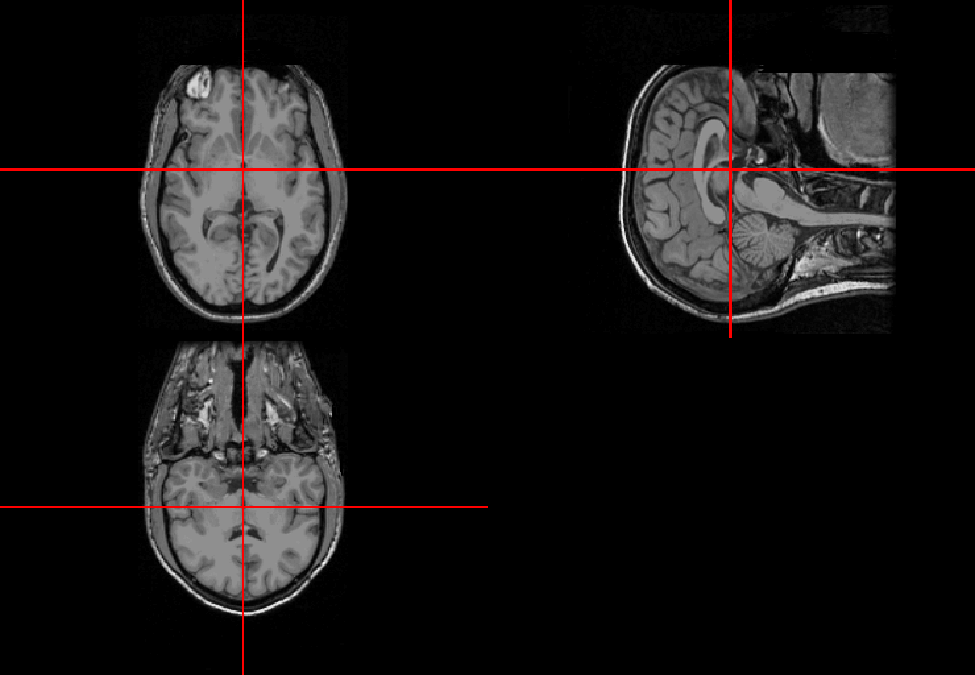
\includegraphics{Freesurfer_files/figure-latex/mri_plot-1} \end{Schunk}

Note, the image is not stored in the ``RPI'' format which is assumed
when displaying using the \pkg{neurobase} \code{ortho2} function. We can
use the \texttt{rpi\_orient} function in fslr (version \(\geq\) 2.4.0)
or \texttt{fslswapdim} to reorient.

\textbackslash{}begin\{Schunk\} \textbackslash{}begin\{Sinput\} L =
fslr::rpi\_orient(img) reoriented\_img = L\$img
\textbackslash{}end\{Sinput\} \textbackslash{}end\{Schunk\}

We see that this function puts this image in the RPI format, which
matches the assumed orientation for \texttt{ortho2}:

\begin{Schunk}
\begin{Sinput}
neurobase::ortho2(reoriented_img, mask = reoriented_img > 40)
\end{Sinput}

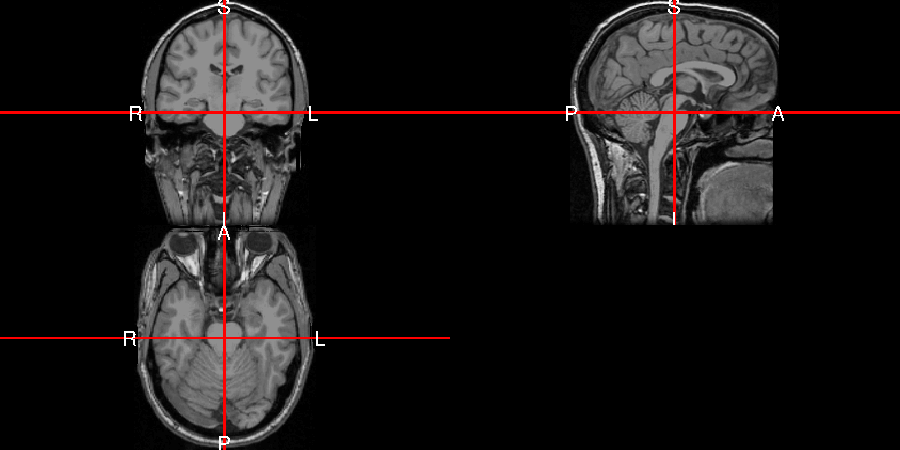
\includegraphics{Freesurfer_files/figure-latex/mri_plot2-1} \end{Schunk}

\subsection{Brain extraction}\label{brain-extraction}

The \code{mri\_watershed} function will segment the brain from the
remainder of the image, such as extra-cranial tissues. Other imaging
software in R have implemented the watershed algorithm, such as
\BIOpkg{EBImage} {[}@EBImage{]}. These methods have not been directly
adapted for MRI nor specifically for brain extraction. In
\pkg{freesurfer}, we can pass in the \code{nifti} object and the output
is a brain-extracted \code{nifti} object.

\begin{Schunk}
\begin{Sinput}
ss = mri_watershed(img)
\end{Sinput}
\end{Schunk}

\begin{Schunk}
\begin{Sinput}
ortho2(ss, mask = ss)
\end{Sinput}
\end{Schunk}\begin{Schunk}

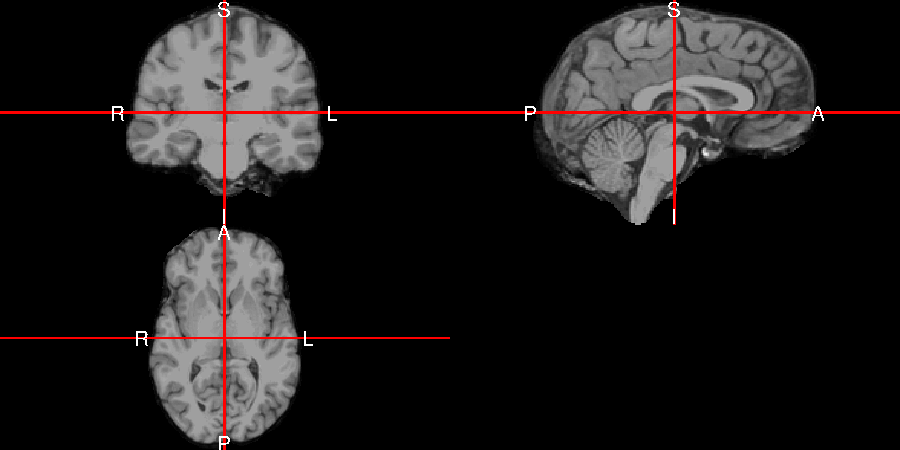
\includegraphics{Freesurfer_files/figure-latex/watershed_plot-1} \end{Schunk}

We see that the area of the skull, eyes, face, and other areas of the
image are removed. We do see some areas that may be part of some of the
membranes between the brain and the skull, but this looks like an
adequate brain extraction for most analyses.

As the result in a \code{nifti} object, we can create a mask by standard
logical operations. As MRI scans are commonly non-zero, the non-zero
areas of the image are the ``brain'':

\begin{Schunk}
\begin{Sinput}
mask = ss > 0
\end{Sinput}
\end{Schunk}

We can then use this mask to perform operations on the image, such as
subsetting.

\subsection{Bias-field correction}

MRI images typically exhibit good contrast between soft tissue classes,
but intensity inhomogeneities in the radio frequency field can cause
differences in the ranges of tissue types at different spatial locations
(e.g.~top versus bottom of the brain). These
inhomogeneities/non-uniformities can cause problems with algorithms
based on histograms, quantiles, or raw intensities
\citep{zhang_segmentation_2001}. Therefore, correction for image
inhomogeneities is a crucial step in many analyses. The Freesurfer
function \code{nu\_correct} performs the non-uniformity correction by
\citet{sled_nonparametric_1998} and the \pkg{freesurfer} function of the
same name will run the correction and return an image.

The Freesurfer \code{nu\_correct} function requires a MNC format
(\url{http://www.bic.mni.mcgill.ca/ServicesSoftware/MINC}). For this to
work, you can convert the \code{nifti} object to a MNC file using
\code{nii2mnc} and pass that file into \code{nu\_correct}. The
\pkg{freesurfer} \code{nu\_correct} function will run the correction and
then convert the output MNC to a NIfTI object.

\begin{Schunk}
\begin{Sinput}
mnc = nii2mnc(reoriented_img)
print(mnc)
\end{Sinput}
\begin{Soutput}
[1] "/var/folders/1s/wrtqcpxn685_zk570bnx9_rr0000gr/T//Rtmpr7Gd1j/filedf9a258a2cc3.mnc"
\end{Soutput}
\begin{Sinput}
nu_from_mnc = nu_correct(file = mnc)
class(nu_from_mnc)
\end{Sinput}
\begin{Soutput}
[1] "nifti"
attr(,"package")
[1] "oro.nifti"
\end{Soutput}
\begin{Sinput}
ortho2(nu_from_mnc, mask = nu_from_mnc > 40)
\end{Sinput}

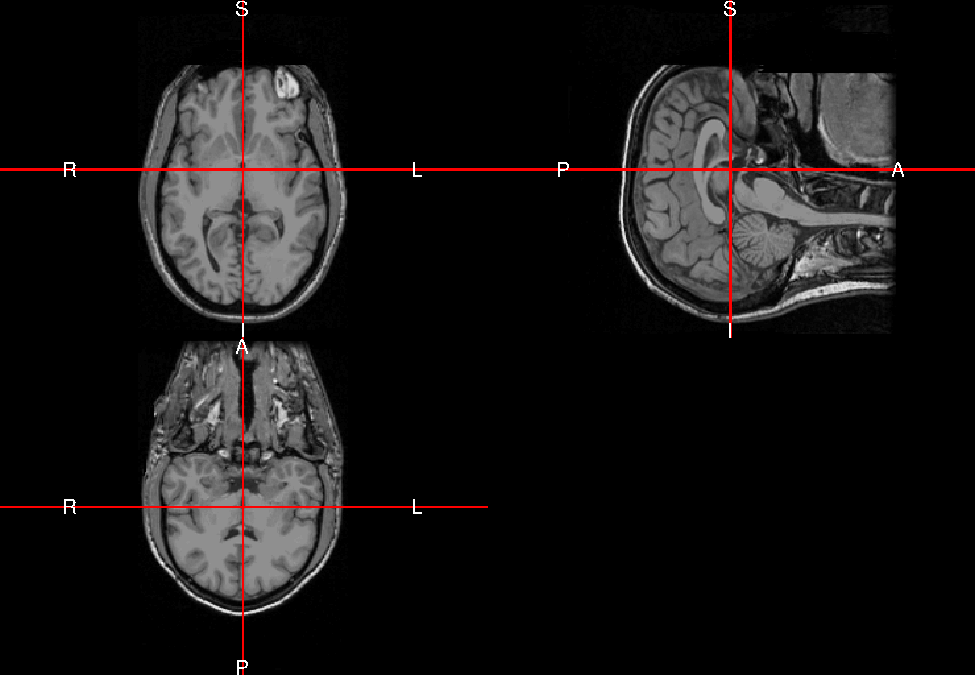
\includegraphics{Freesurfer_files/figure-latex/nu_correct_mcn2nii-1} \end{Schunk}

If you pass in a \code{nifti} object in directly into
\texttt{nu\_correct}, the function will automatically convert any NIfTI
input files, and then run the correction. We can also pass in a mask
(generated from above) to run the correction only the areas of the
brain.

\begin{Schunk}
\begin{Sinput}
nu_masked = nu_correct(file = reoriented_img, mask = mask)
class(nu_masked)
\end{Sinput}
\begin{Soutput}
[1] "nifti"
attr(,"package")
[1] "oro.nifti"
\end{Soutput}
\end{Schunk}

Overall, this correction is a way to make the intensities of the brain
more homogeneous spatially. This method is different from that
implemented in FSL (and therefore \pkg{fslr}), so it provides an
alternative method to the R user than currently available.

\subsection{Label files}\label{label-files}

Here we will read a label file for the left hemisphere cortex:

\begin{Schunk}
\begin{Sinput}
file = file.path(fs_subj_dir(), "bert", "label", "lh.cortex.label")
out = read_fs_label(file)
head(out)
\end{Sinput}
\begin{Soutput}
  vertex_num r_coord  a_coord s_coord        value
1          0 -12.882 -102.449  -9.782 0.0000000000
2          1 -13.331 -102.518  -9.829 0.0000000000
3          2 -13.637 -102.514 -10.077 0.0000000000
4          3 -13.031 -102.596 -10.024 0.0000000000
5          4 -13.331 -102.510 -10.254 0.0000000000
6          5 -13.610 -102.483 -10.295 0.0000000000
\end{Soutput}
\end{Schunk}

The coordinates are mostly used in these files, not the value assigned.
They can be used for registration as well.

\subsection{Additional Features}\label{additional-features}

For the initial release, we did not implement a method to read the
annotation files and other surface-based files that Freesurfer uses.
Reading in these files are planned for a future release. Freesurfer can
also analyze diffusion tensor imaging (DTI) data and some of the
functions have been adapted for \pkg{freesurfer} but have not been
thoroughly tested.

\subsection{Conclusion}\label{conclusion}

The neuroimaging community has developed a large collection of tools for
image processing and analysis. Some of the fundamental functionality of
neuroimage processing is being added to R packages, such as our previous
work porting FSL to R using \pkg{fslr} and the actively-developed GitHub
\pkg{ANTsR} package. Additional third-party software still has
additional functionality that is not present in R, such as the
surface-based registration and processing of Freesurfer. We present
\pkg{freesurfer} to bridge this gap and provide R users functions from
Freesurfer. Interfacing R with existing, powerful software provides
users with thoroughly-tested software and an additional community of
users, which would not be available if the functions were rewritten in
R. Although this external software dependency may not be an advantage
for the software, it benefits from the years of previous testing.

There has been an increasing popularity of similar interfacing of tools
within the Python community such as Nipype
\citep{gorgolewski_nipype:_2011}
(\url{https://qa.debian.org/popcon.php?package=nipype}). As many users
of R may not have experience with Python or bash scripting, we believe
\pkg{freesurfer} provides a lower threshold for use in the R community.

Most importantly, as \pkg{freesurfer} is based on the R framework, all
the benefits of using R are available, such as dynamic documents, Shiny
applications, customized figures, and state-of-the-art statistical
methods. These benefits provide unique functionality compared to other
software packages for neuroimaging.

\subsection{Reproducibility}\label{reproducibility}

This paper was generated using the \CRANpkg{rticles} package
{[}@rticles{]}. All necessary code to generate this report is located
at: \url{https://github.com/muschellij2/fs_paper}.

\bibliography{RJreferences}

\address{%
John Muschelli\\
Johns Hopkins Bloomberg School of Public Health\\
Department of Biostatistics\\ 615 N Wolfe St, Baltimore, MD, 21205\\
}
\href{mailto:jmuschel@jhsph.edu}{\nolinkurl{jmuschel@jhsph.edu}}

\address{%
Elizabeth M. Sweeney\\
Rice University\\
Department of Statistics\\ 6100 Main St, Duncan Hall, Houston, TX, 77005\\
}
\href{mailto:ems15@rice.edu}{\nolinkurl{ems15@rice.edu}}

\address{%
Ciprian M. Crainiceanu\\
Johns Hopkins Bloomberg School of Public Health\\
Department of Biostatistics\\ 615 N Wolfe St, Baltimore, MD, 21205\\
}
\href{mailto:ccraini1@jhu.edu}{\nolinkurl{ccraini1@jhu.edu}}

